% Preamble
\documentclass [a4paper,12pt,oneside,final,titlepage]{article}
\usepackage[left=35mm,top=35mm,right=26mm,bottom=15mm]{geometry}

\usepackage{listings}
\usepackage{graphicx}
\usepackage{color}
\usepackage{float}
\usepackage{natbib}
\usepackage{fancyhdr}


\pagestyle{fancy}
%\fancypagestyle{IHA-fancy-style}{%
  \fancyhf{}% Clear header and footer
  \fancyhead[LE,LO]{Hessler}
  \fancyhead[RO,RE]{\LaTeX}
  \fancyfoot[CO,CE]{Page \thepage}
%  \fancypagestyle{plain}{\pagestyle{fancy}}
%  %\fancyfoot[C]{\thepage\ of \pageref{LastPage}}% Custom footer
%  \renewcommand{\headrulewidth}{0.0pt}% Line at the header visible
%  \renewcommand{\footrulewidth}{0.4pt}% Line at the footer visible
%%}



\definecolor{dkgreen}{rgb}{0,0.6,0}
\definecolor{gray}{rgb}{0.5,0.5,0.5}
\definecolor{mauve}{rgb}{0.58,0,0.82}

%\setcounter{topnumber}{2}
%\setcounter{bottomnumber}{2}
%\setcounter{totalnumber}{4}
%\renewcommand{\topfraction}{0.85}
%\renewcommand{\bottomfraction}{0.85}
%\renewcommand{\textfraction}{0.15}
%\renewcommand{\floatpagefraction}{0.8}
%\renewcommand{\textfraction}{0.1}
%\setlength{\floatsep}{5pt plus 2pt minus 2pt}
%\setlength{\textfloatsep}{5pt plus 2pt minus 2pt}
%\setlength{\intextsep}{5pt plus 2pt minus 2pt}

\lstset{frame=tb,
  language=Java,
  aboveskip=3mm,
  belowskip=3mm,
  showstringspaces=false,
  columns=flexible,
  basicstyle={\small\ttfamily},
  numbers=none,
  numberstyle=\tiny\color{gray},
  keywordstyle=\color{blue},
  commentstyle=\color{dkgreen},
  stringstyle=\color{mauve},
  breaklines=true,
  breakatwhitespace=true,
  tabsize=3
}

\setlength{\voffset}{-0.5in}

\title{An Implementation of Java Native Interface (JNI) to Replace a Socket}
\author{Brandon Hessler  \\
	Penn State - World Campus  \\
	Enterprise Integration \\
	SWENG568 Section 1 \\
	Program: Software Engineering M.S. \\
	}

\date{\today} 

\begin{document}
	\maketitle
	\tableofcontents
	
	\section{Project Introduction}
	
	\subsection{Business View of the Integration Needs }

	
	\section{Workflows or Process Flows Design (e.g., Integration logic across integrated applications)}
	
	\subsection{Data Flow}
	\subsection{Control Flow}
	

	\section{Integration Design (i.e., Approach to implementing the identified integration logic)}

	\subsection{Architecture Models (An architectural model is an overall structure of your systems, which provides the general relationship of highlevel components across integrated applications.) }

	\subsection{Functional Models (A functional model is essentially a list of specific functions to support a given integration need. It provides
an overview of the essential functions supported by integrated applications and how they are related.) }
	

	\section{Implementation and Programming}
	
	\section{Bibliography}


	\begin{itemize}
	\item JAX-WS \\
	I used JAX and the @WebService annotations in order create a document style web service. JAX-WS is an easier way for me to implement the SOAP style functionality but with an easier time than doing so without an API. JAX-WS is an easy and secure way for Java to implement the RESTful Web Service that it seems most people use these days.
	\item wsgen \\
	Using wsgen was not an easy thing to accomplish. I had to spend a lot of time trying to throw different commands at this in order to get it to work. The biggest problem was that I was not calling the wsgen function from the correct place, I was calling it from the code path instead of the compiled code path (in the out folder). This generated the two java classes I needed in order to aid with the deploement of the Web Server. One is able to accomplish the same task by writing it by hand (I realized this after) and it would have been much less time consuming in my case. But for a complicated Web Server with a lot of calls, I could see how this could speed things up tremendously. Screenshot of me running this is in Figure \ref{fig:cmd}.

	%\begin{figure}[htp]
	%	\centering
	%	\vspace{20pt}
	%	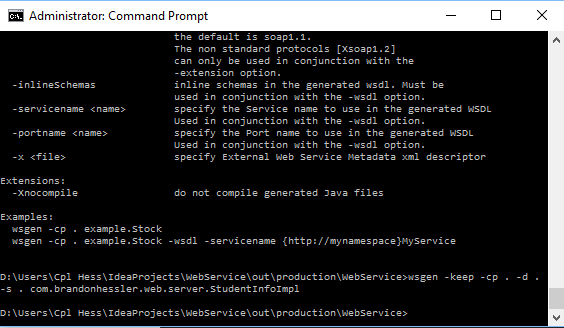
\includegraphics[height=55mm]{cmd}
	%	\caption{Command Prompt for the wsgen code generation}
	%	\label{fig:cmd}
%	\end{figure}
	
	\vspace{5mm}

	\item w3c dom \\
	I almost decided not to do this step since I already had the web service working and could take things from a file and send it over the Web Service before I started to use it. But it didn't quite sit right with me only having a hard coded string that would be sent. I instead wanted to use the XML file that was given to us in the lesson to find the correct student to send over the network. Once I decided this I needed to learn how to traverse an XML document in Java without parsing it into one or more objects. Obviously this would have been much easier, but most likely an unnecessary step in the real world. It makes much more sense to look through the student data that is already in the XML file (produced by whomever) and send the requested data as is so that they can parse what they need from it. Through my research I learned that the easiest way to do this was with the w3c dom package, which lets you traverse the Nodes of the XML file and get the requested data. That data is then sent over the Web Service and received by the client.
	\end{itemize}


	
	
\end{document}